% Options for packages loaded elsewhere
\PassOptionsToPackage{unicode}{hyperref}
\PassOptionsToPackage{hyphens}{url}
%
\documentclass[
]{article}
\usepackage{amsmath,amssymb}
\usepackage{iftex}
\ifPDFTeX
  \usepackage[T1]{fontenc}
  \usepackage[utf8]{inputenc}
  \usepackage{textcomp} % provide euro and other symbols
\else % if luatex or xetex
  \usepackage{unicode-math} % this also loads fontspec
  \defaultfontfeatures{Scale=MatchLowercase}
  \defaultfontfeatures[\rmfamily]{Ligatures=TeX,Scale=1}
\fi
\usepackage{lmodern}
\ifPDFTeX\else
  % xetex/luatex font selection
\fi
% Use upquote if available, for straight quotes in verbatim environments
\IfFileExists{upquote.sty}{\usepackage{upquote}}{}
\IfFileExists{microtype.sty}{% use microtype if available
  \usepackage[]{microtype}
  \UseMicrotypeSet[protrusion]{basicmath} % disable protrusion for tt fonts
}{}
\makeatletter
\@ifundefined{KOMAClassName}{% if non-KOMA class
  \IfFileExists{parskip.sty}{%
    \usepackage{parskip}
  }{% else
    \setlength{\parindent}{0pt}
    \setlength{\parskip}{6pt plus 2pt minus 1pt}}
}{% if KOMA class
  \KOMAoptions{parskip=half}}
\makeatother
\usepackage{xcolor}
\usepackage[margin=1in]{geometry}
\usepackage{graphicx}
\makeatletter
\def\maxwidth{\ifdim\Gin@nat@width>\linewidth\linewidth\else\Gin@nat@width\fi}
\def\maxheight{\ifdim\Gin@nat@height>\textheight\textheight\else\Gin@nat@height\fi}
\makeatother
% Scale images if necessary, so that they will not overflow the page
% margins by default, and it is still possible to overwrite the defaults
% using explicit options in \includegraphics[width, height, ...]{}
\setkeys{Gin}{width=\maxwidth,height=\maxheight,keepaspectratio}
% Set default figure placement to htbp
\makeatletter
\def\fps@figure{htbp}
\makeatother
\setlength{\emergencystretch}{3em} % prevent overfull lines
\providecommand{\tightlist}{%
  \setlength{\itemsep}{0pt}\setlength{\parskip}{0pt}}
\setcounter{secnumdepth}{-\maxdimen} % remove section numbering
\usepackage{booktabs}
\usepackage{longtable}
\usepackage{array}
\usepackage{multirow}
\usepackage{wrapfig}
\usepackage{float}
\usepackage{colortbl}
\usepackage{pdflscape}
\usepackage{tabu}
\usepackage{threeparttable}
\usepackage{threeparttablex}
\usepackage[normalem]{ulem}
\usepackage{makecell}
\usepackage{xcolor}
\ifLuaTeX
  \usepackage{selnolig}  % disable illegal ligatures
\fi
\IfFileExists{bookmark.sty}{\usepackage{bookmark}}{\usepackage{hyperref}}
\IfFileExists{xurl.sty}{\usepackage{xurl}}{} % add URL line breaks if available
\urlstyle{same}
\hypersetup{
  pdftitle={Gráficos Presentación Renca},
  pdfauthor={Cristóbal Ortiz},
  hidelinks,
  pdfcreator={LaTeX via pandoc}}

\title{Gráficos Presentación Renca}
\author{Cristóbal Ortiz}
\date{2023-07-14}

\begin{document}
\maketitle

\hypertarget{caracterizaciuxf3n-de-macrozonas-y-poblaciuxf3n}{%
\section{1. Caracterización de macrozonas y
población}\label{caracterizaciuxf3n-de-macrozonas-y-poblaciuxf3n}}

\hypertarget{macrozonas}{%
\subsection{Macrozonas}\label{macrozonas}}

\begin{flushleft}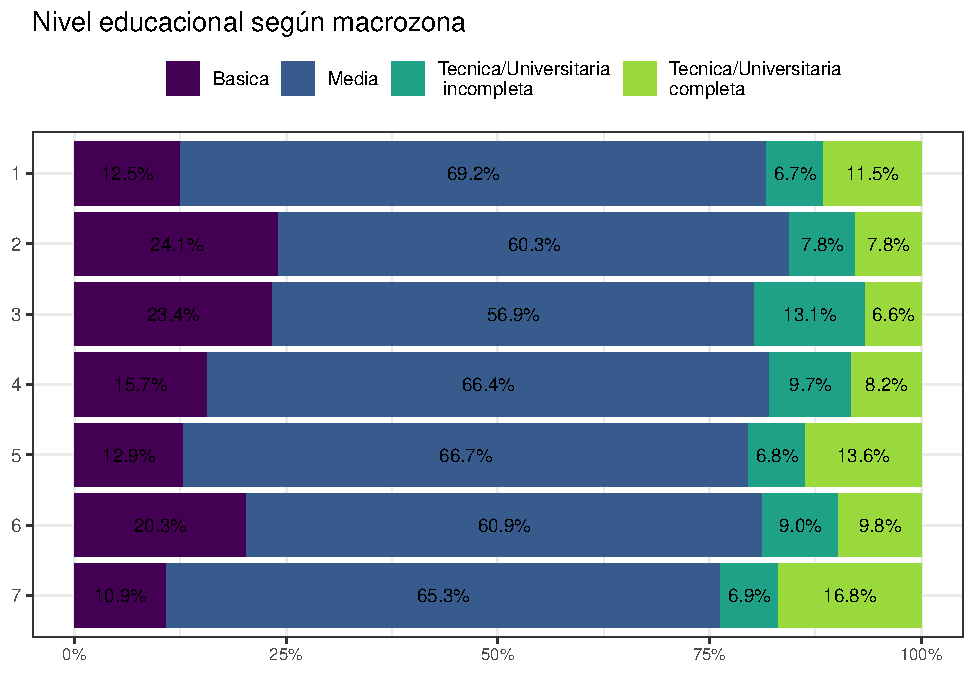
\includegraphics{presentacion-renca_files/figure-latex/educ-zona-1} \end{flushleft}

\begin{flushleft}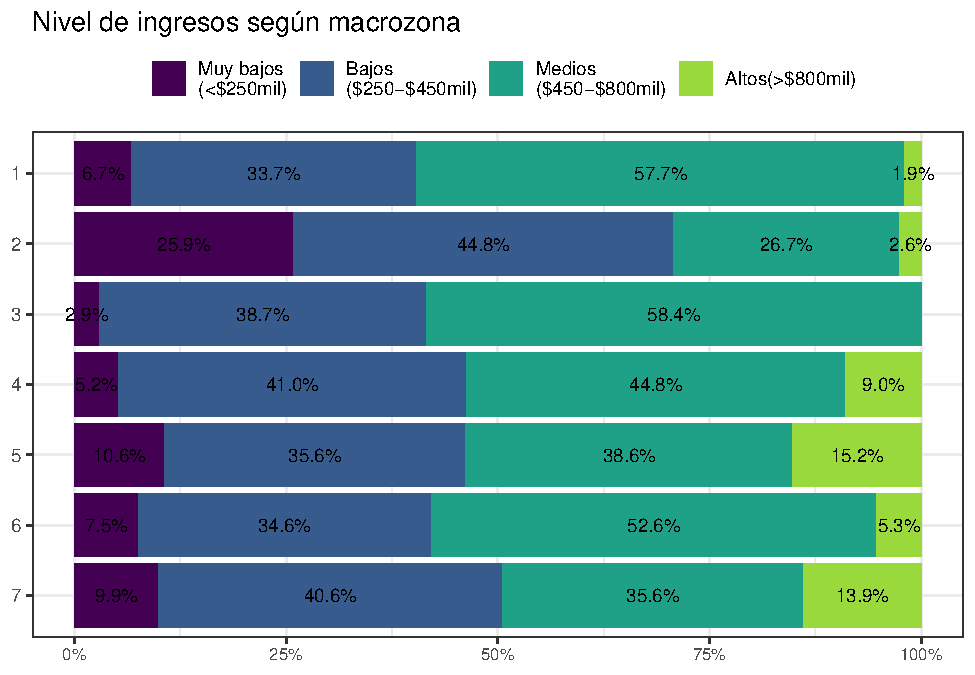
\includegraphics{presentacion-renca_files/figure-latex/ingr-zona-1} \end{flushleft}

\hypertarget{la-cohesiuxf3n-en-perspectiva-comparada}{%
\section{2. La cohesión en perspectiva
comparada}\label{la-cohesiuxf3n-en-perspectiva-comparada}}

\hypertarget{indicadores-de-cohesiuxf3n-barrial-horizontal}{%
\subsection{2.1. Indicadores de cohesión barrial
horizontal}\label{indicadores-de-cohesiuxf3n-barrial-horizontal}}

\hypertarget{a.-apego-al-barrio}{%
\subsubsection{a. Apego al barrio}\label{a.-apego-al-barrio}}

\begin{flushleft}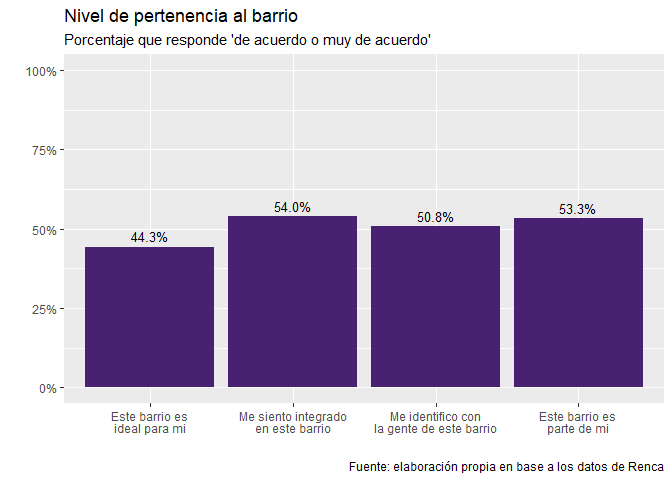
\includegraphics{presentacion-renca_files/figure-latex/spb-renca-1} \end{flushleft}

\begin{flushleft}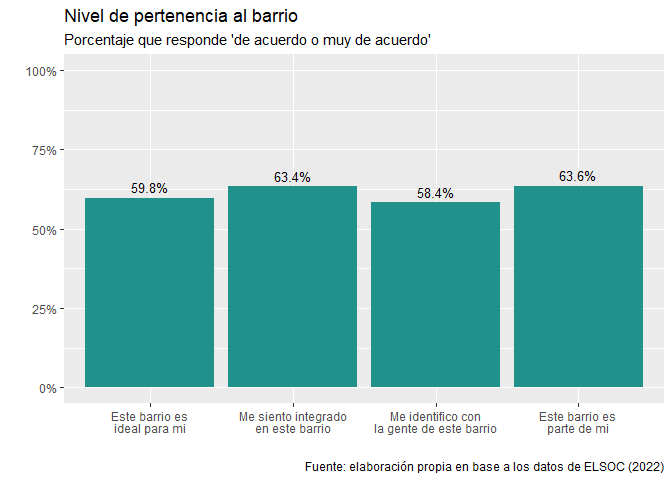
\includegraphics{presentacion-renca_files/figure-latex/spb-ams-1} \end{flushleft}

\hypertarget{b.-arraigo-fuxedsico}{%
\subsubsection{b. Arraigo físico}\label{b.-arraigo-fuxedsico}}

\begin{flushleft}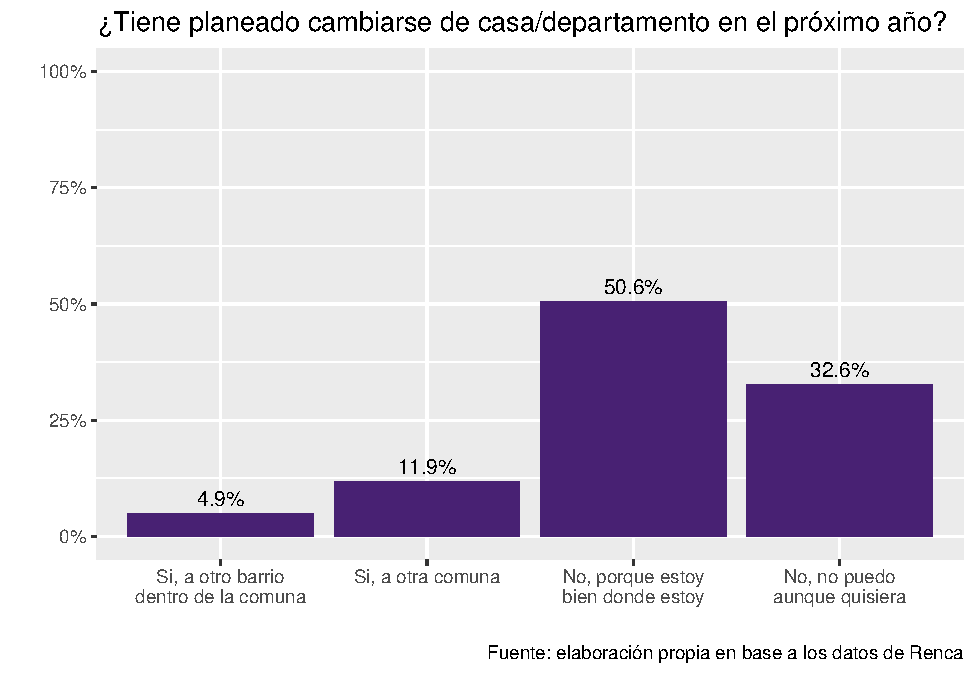
\includegraphics{presentacion-renca_files/figure-latex/arraigo-renca-1} \end{flushleft}

\begin{verbatim}
## x <numeric> 
## # total N=800 valid N=760 mean=2.94 sd=0.90
## 
## Value |   N | Raw % | Valid % | Cum. %
## --------------------------------------
##     1 |  73 |  9.12 |    9.61 |   9.61
##     2 | 115 | 14.37 |   15.13 |  24.74
##     3 | 357 | 44.62 |   46.97 |  71.71
##     4 | 215 | 26.88 |   28.29 | 100.00
##  <NA> |  40 |  5.00 |    <NA> |   <NA>
\end{verbatim}

\begin{flushleft}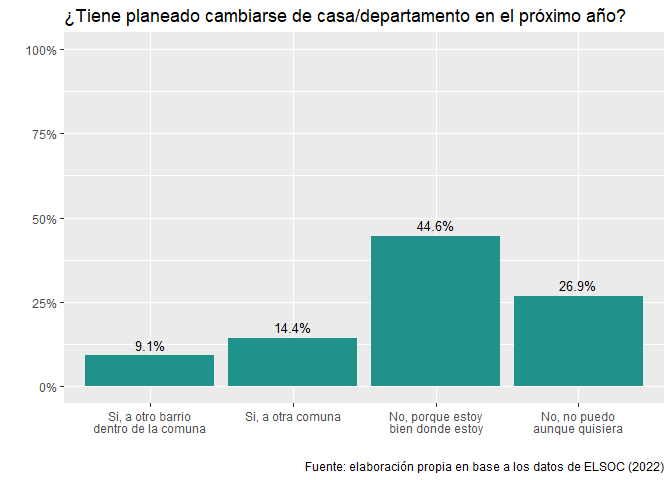
\includegraphics{presentacion-renca_files/figure-latex/arraigo-ams-1} \end{flushleft}

\hypertarget{c.-sociabilidad-barrial}{%
\subsubsection{c.~Sociabilidad barrial}\label{c.-sociabilidad-barrial}}

\begin{flushleft}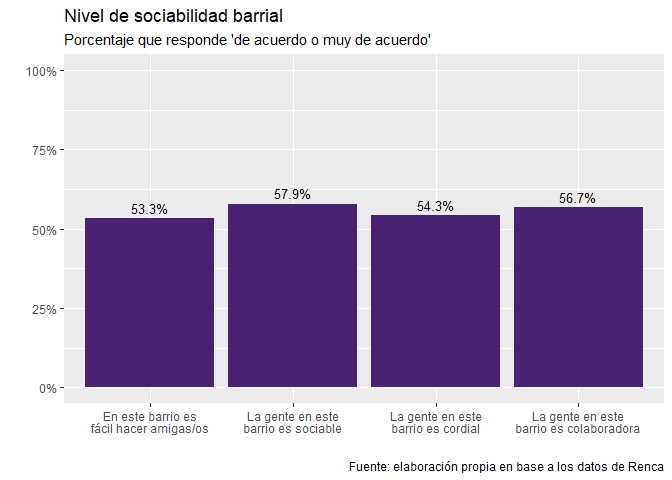
\includegraphics{presentacion-renca_files/figure-latex/soci-renca-1} \end{flushleft}

\begin{flushleft}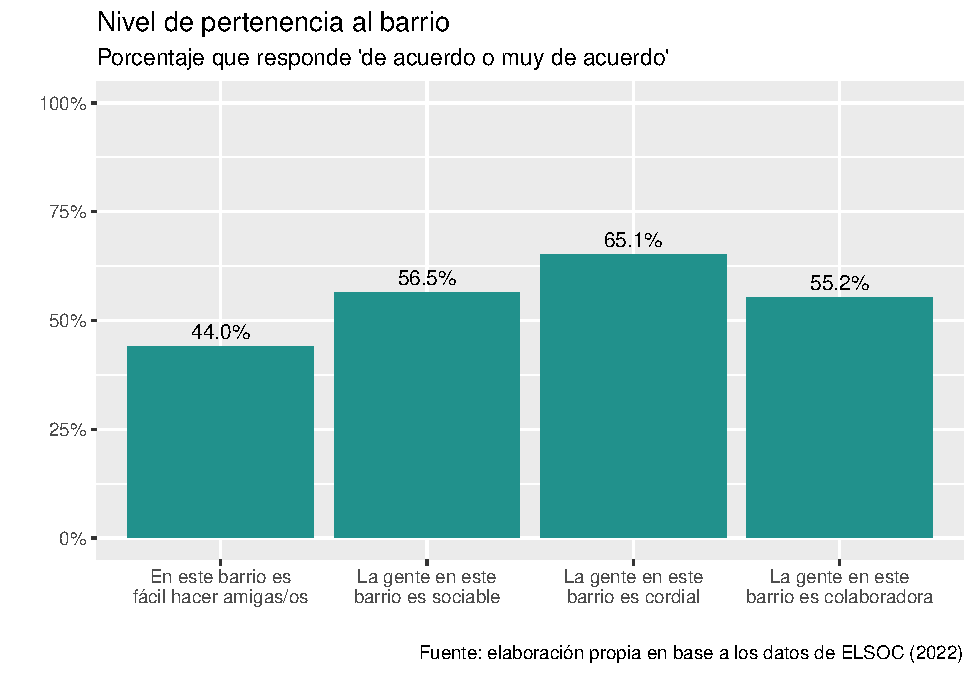
\includegraphics{presentacion-renca_files/figure-latex/soci-ams-1} \end{flushleft}

\hypertarget{d.-confianza-en-vecinos}{%
\subsubsection{d.~Confianza en vecinos}\label{d.-confianza-en-vecinos}}

\begin{flushleft}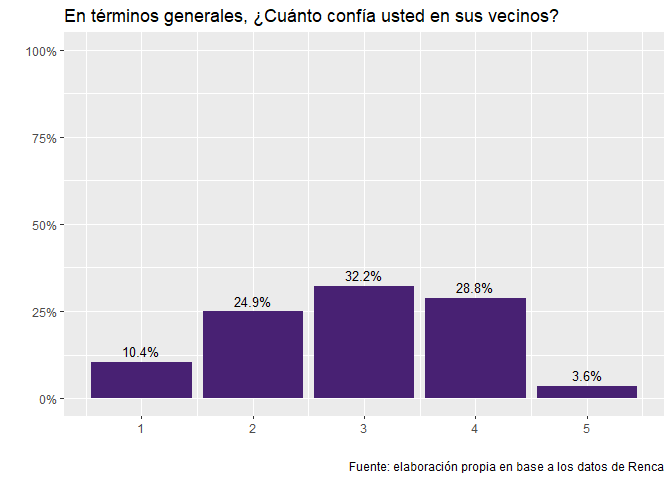
\includegraphics{presentacion-renca_files/figure-latex/conf-renca-1} \end{flushleft}

\begin{flushleft}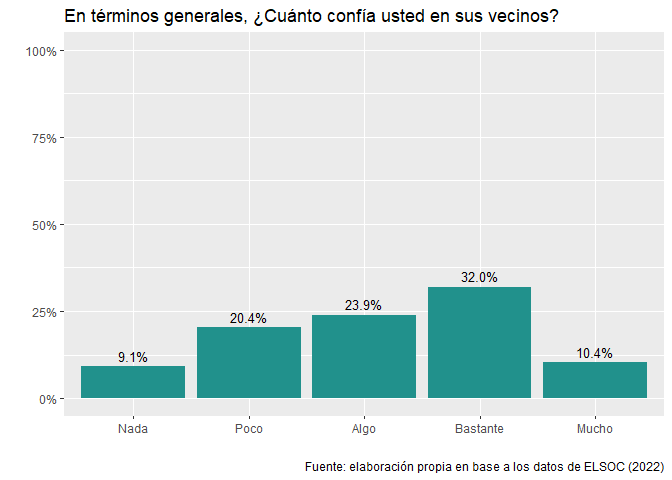
\includegraphics{presentacion-renca_files/figure-latex/conf-ams-1} \end{flushleft}

\hypertarget{e.-participaciuxf3n-local}{%
\subsubsection{e. Participación
local**}\label{e.-participaciuxf3n-local}}

\hypertarget{f.-apoyo-social}{%
\subsubsection{f.~Apoyo social}\label{f.-apoyo-social}}

\begin{flushleft}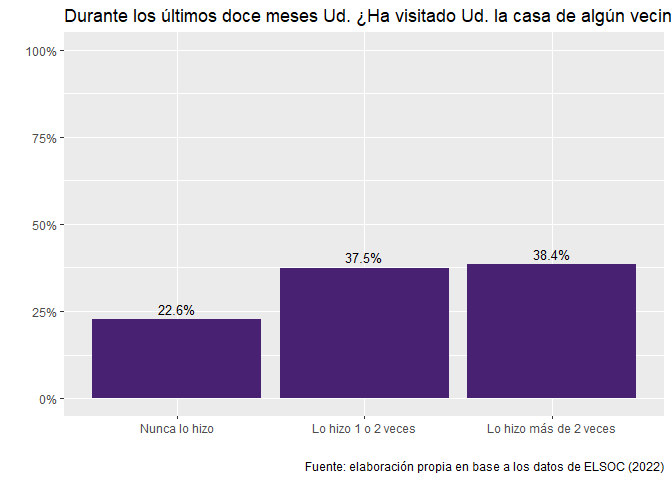
\includegraphics{presentacion-renca_files/figure-latex/apoy-renca-1} \end{flushleft}

\begin{flushleft}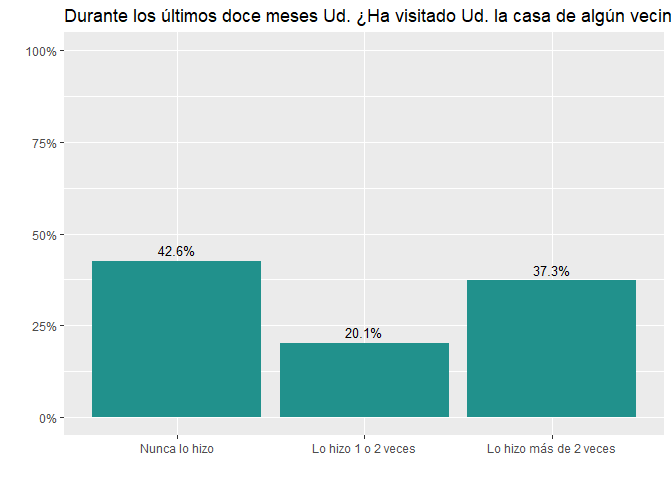
\includegraphics{presentacion-renca_files/figure-latex/apoy-ams-1} \end{flushleft}

\hypertarget{cohesiuxf3n-barrial-vertical}{%
\subsection{2.2. Cohesión barrial
vertical}\label{cohesiuxf3n-barrial-vertical}}

\hypertarget{a.-confianza-en-autoridades-e-instituciones-de-la-comuna}{%
\subsubsection{a. Confianza en autoridades e instituciones de la
comuna}\label{a.-confianza-en-autoridades-e-instituciones-de-la-comuna}}

\begin{flushleft}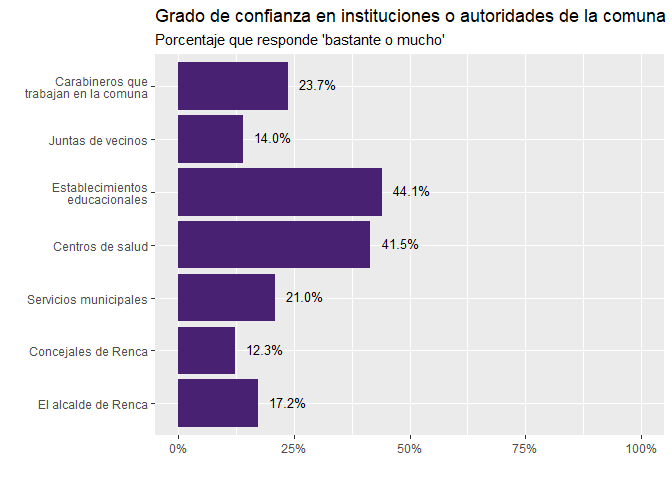
\includegraphics{presentacion-renca_files/figure-latex/conf-aut-renca-1} \end{flushleft}

\hypertarget{b.-participaciuxf3n-en-organizaciones-de-la-comuna}{%
\subsubsection{b. Participación en organizaciones de la
comuna}\label{b.-participaciuxf3n-en-organizaciones-de-la-comuna}}

\begin{flushleft}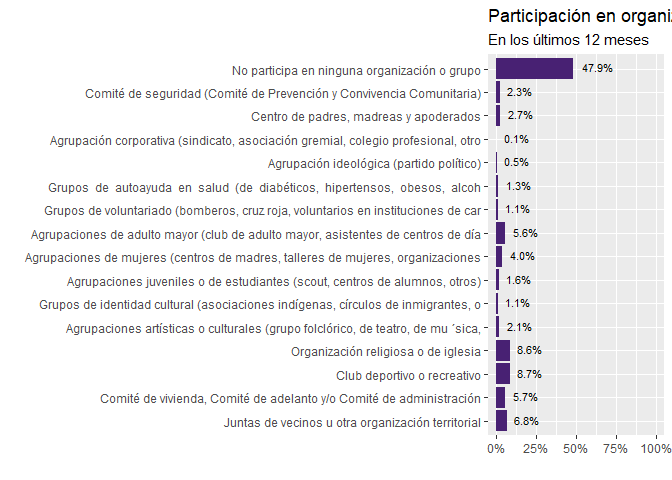
\includegraphics{presentacion-renca_files/figure-latex/part-org-renca-1} \end{flushleft}

\begin{flushleft}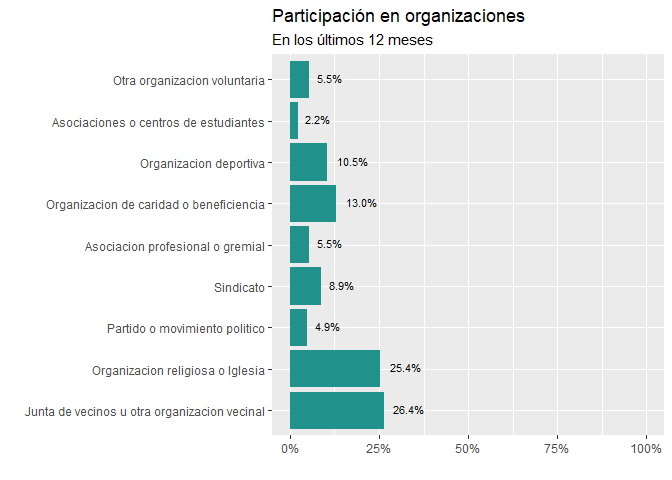
\includegraphics{presentacion-renca_files/figure-latex/part-org-ams-1} \end{flushleft}

\hypertarget{c.-activida-cuxedvica}{%
\subsubsection{c.~Activida cívica}\label{c.-activida-cuxedvica}}

\begin{verbatim}
## Asistido a alguna reunión donde se traten temas de interés público o comunitario (x) <numeric> 
## # total N=982 valid N=982 mean=1.72 sd=0.49
## 
## Value |        Label |   N | Raw % | Valid % | Cum. %
## -----------------------------------------------------
##     1 |           Sí | 291 | 29.63 |   29.63 |  29.63
##     2 |           No | 673 | 68.53 |   68.53 |  98.17
##     3 | NS (no leer) |  16 |  1.63 |    1.63 |  99.80
##     4 | NR (no leer) |   2 |  0.20 |    0.20 | 100.00
##  <NA> |         <NA> |   0 |  0.00 |    <NA> |   <NA>
\end{verbatim}

\begin{flushleft}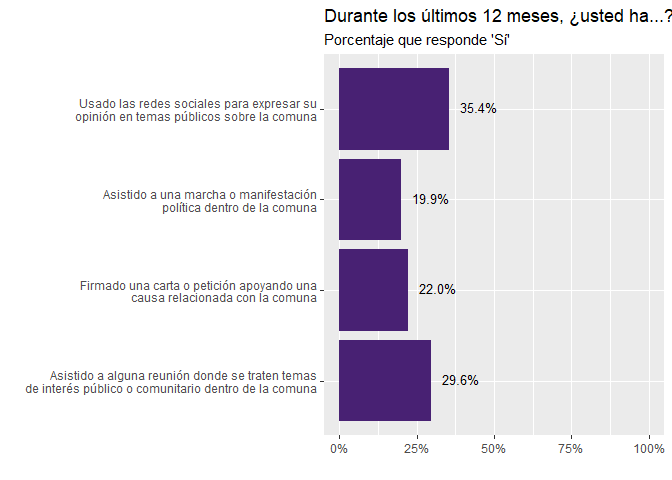
\includegraphics{presentacion-renca_files/figure-latex/activ-renca-1} \end{flushleft}

\hypertarget{tolerancia-a-la-diversidad}{%
\subsection{2.3. Tolerancia a la
diversidad}\label{tolerancia-a-la-diversidad}}

\begin{flushleft}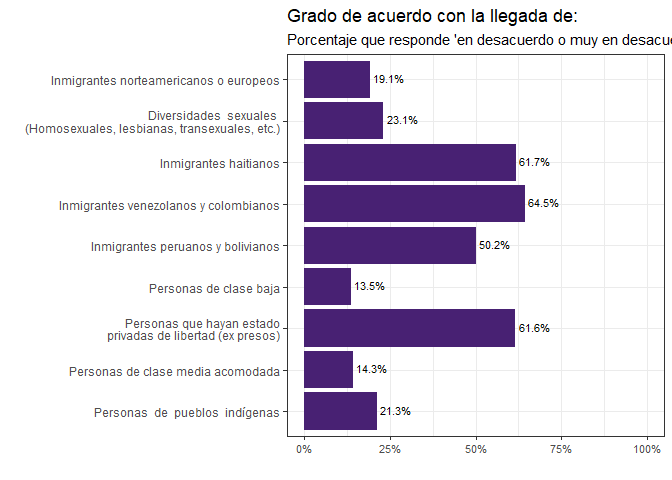
\includegraphics{presentacion-renca_files/figure-latex/dive-gral-1} \end{flushleft}

\begin{flushleft}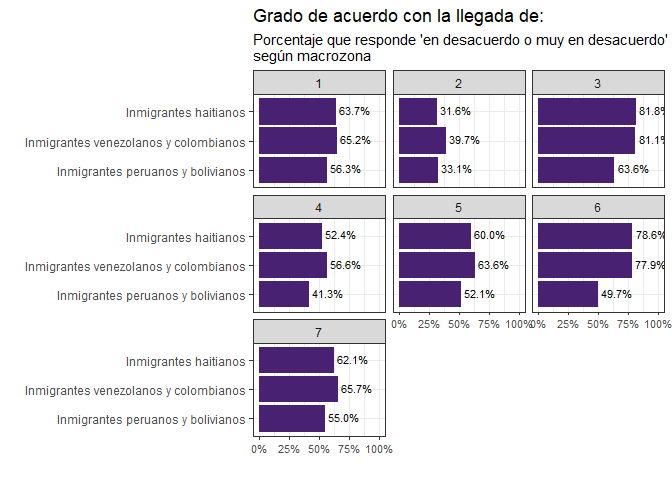
\includegraphics{presentacion-renca_files/figure-latex/dive-zona-1} \end{flushleft}

\hypertarget{perfiles-de-cohesiuxf3n-barrial-en-renca}{%
\section{3. Perfiles de cohesión barrial en
Renca}\label{perfiles-de-cohesiuxf3n-barrial-en-renca}}

\begin{flushleft}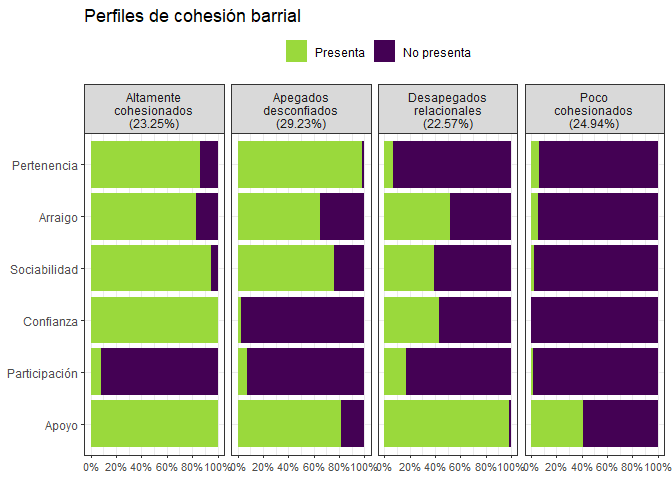
\includegraphics{presentacion-renca_files/figure-latex/tipos-cb-1} \end{flushleft}

\begin{flushleft}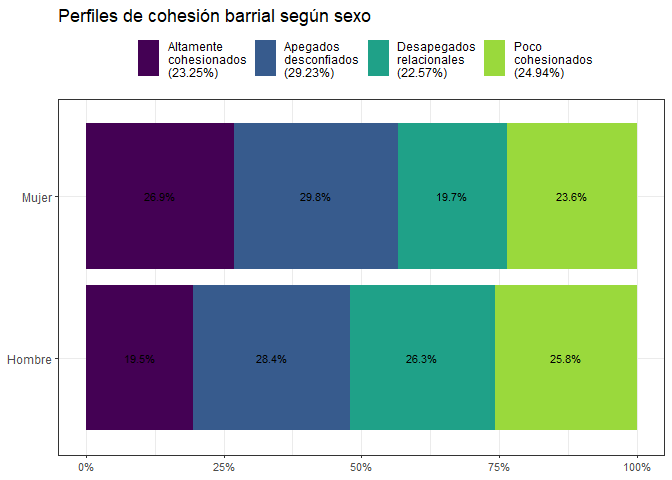
\includegraphics{presentacion-renca_files/figure-latex/tipos-sexo-1} \end{flushleft}

\begin{flushleft}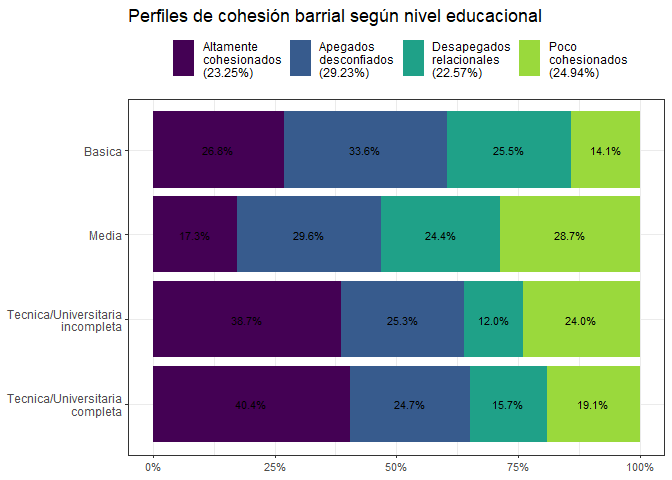
\includegraphics{presentacion-renca_files/figure-latex/tipos-educ-1} \end{flushleft}

\begin{flushleft}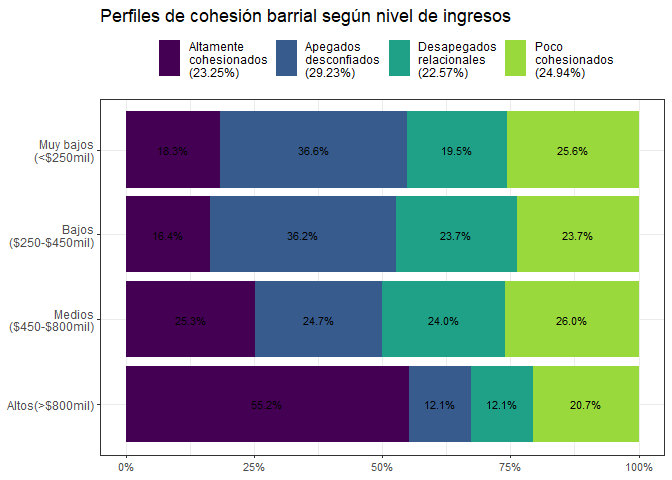
\includegraphics{presentacion-renca_files/figure-latex/tipos-ingr-1} \end{flushleft}

\begin{flushleft}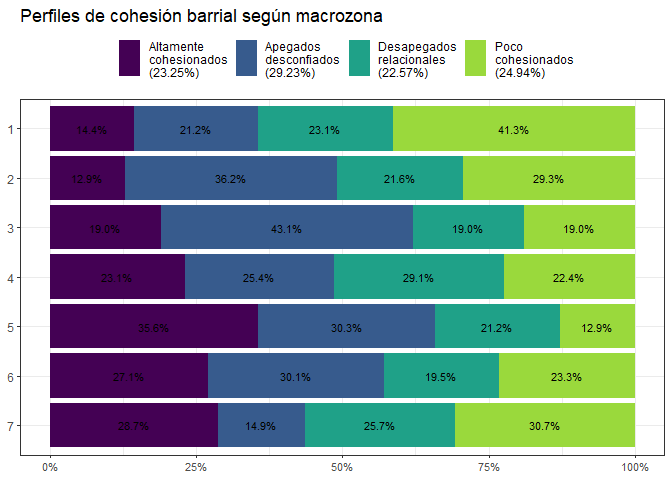
\includegraphics{presentacion-renca_files/figure-latex/tipos-zonas-1} \end{flushleft}

\begin{flushleft}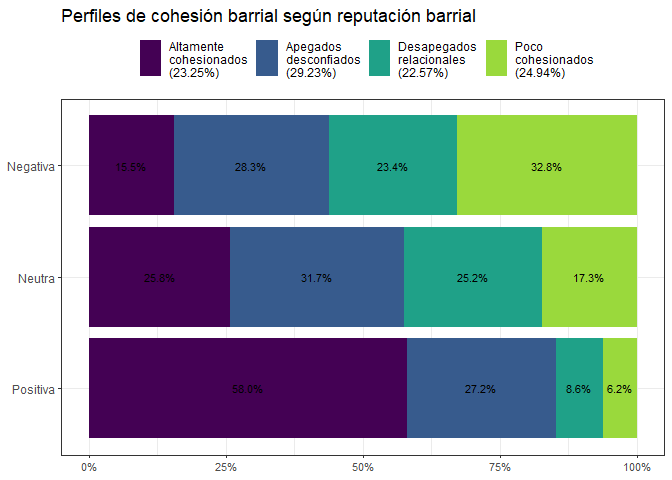
\includegraphics{presentacion-renca_files/figure-latex/tipos-repb-1} \end{flushleft}

\begin{flushleft}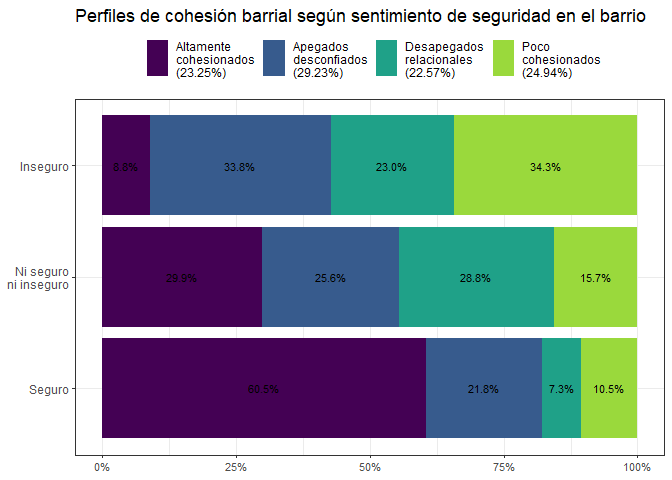
\includegraphics{presentacion-renca_files/figure-latex/tipos-segu-1} \end{flushleft}

\hypertarget{factores-relacionados-a-la-cohesiuxf3n}{%
\section{4. Factores relacionados a la
cohesión}\label{factores-relacionados-a-la-cohesiuxf3n}}

\hypertarget{seguridad}{%
\subsection{4.2. Seguridad}\label{seguridad}}

\begin{flushleft}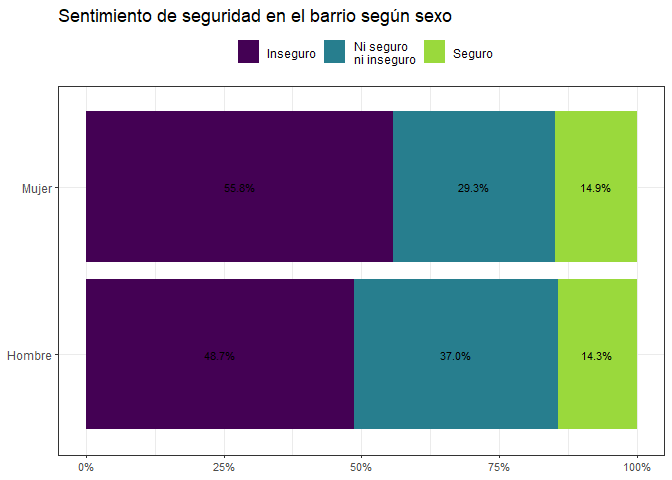
\includegraphics{presentacion-renca_files/figure-latex/segu-sexo-1} \end{flushleft}

\begin{flushleft}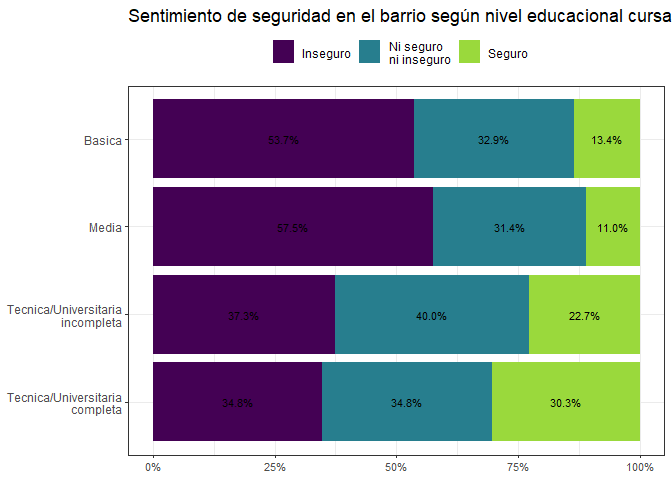
\includegraphics{presentacion-renca_files/figure-latex/segu-educ-1} \end{flushleft}

\begin{flushleft}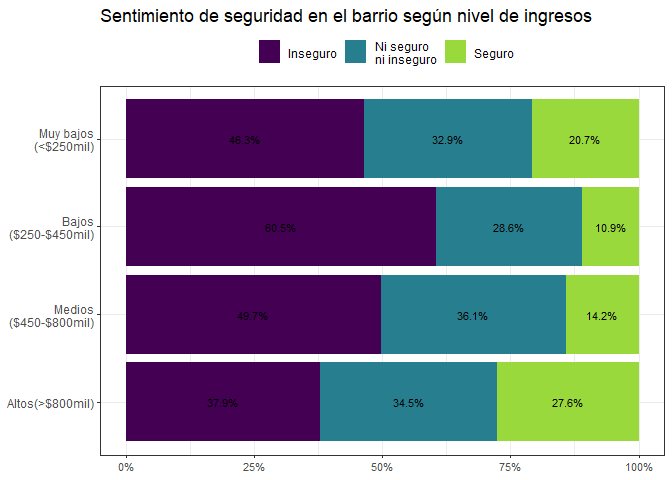
\includegraphics{presentacion-renca_files/figure-latex/segu-ingr-1} \end{flushleft}

\begin{flushleft}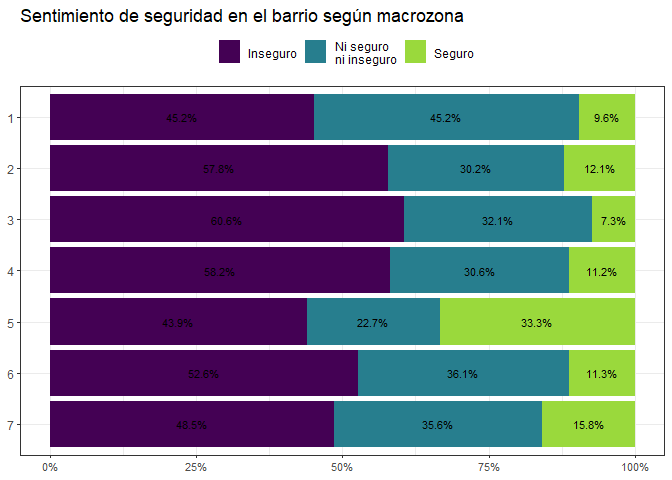
\includegraphics{presentacion-renca_files/figure-latex/segu-zonas-1} \end{flushleft}

\hypertarget{reputaciuxf3n}{%
\subsection{4.3. Reputación}\label{reputaciuxf3n}}

\begin{flushleft}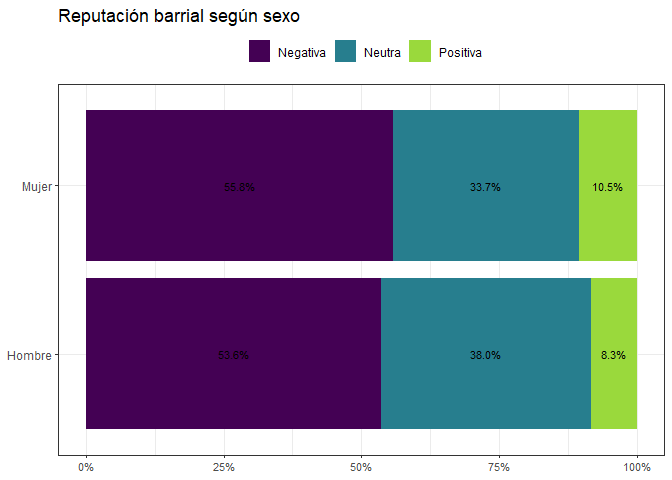
\includegraphics{presentacion-renca_files/figure-latex/repb-sexo-1} \end{flushleft}

\begin{flushleft}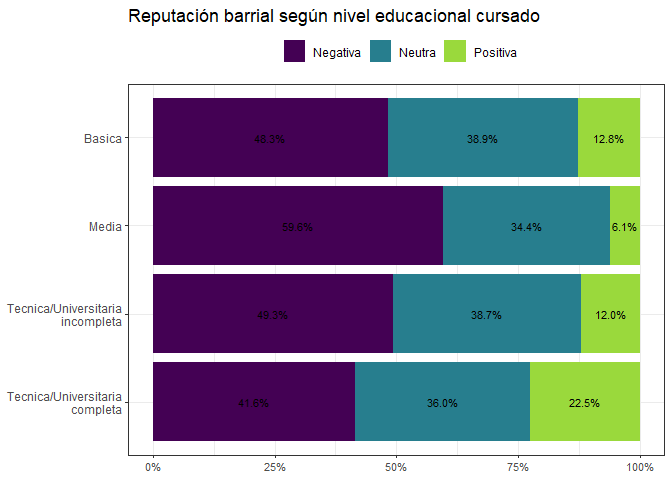
\includegraphics{presentacion-renca_files/figure-latex/repb-educ-1} \end{flushleft}

\begin{flushleft}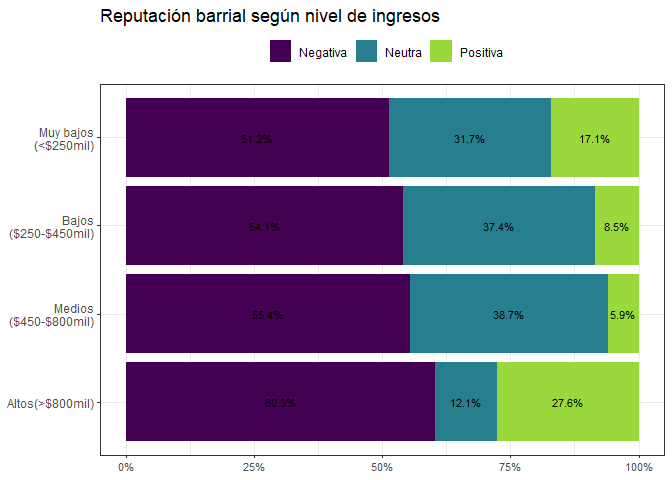
\includegraphics{presentacion-renca_files/figure-latex/repb-ingr-1} \end{flushleft}

\begin{flushleft}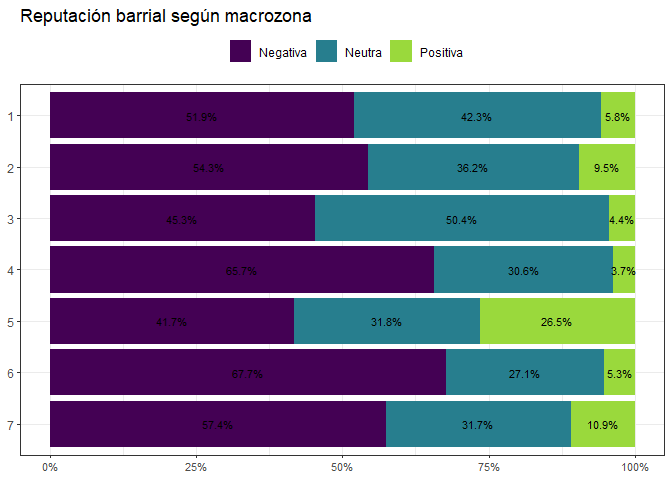
\includegraphics{presentacion-renca_files/figure-latex/repb-zonas-1} \end{flushleft}

\hypertarget{evaluaciuxf3n-del-municipio}{%
\section{5. Evaluación del
municipio}\label{evaluaciuxf3n-del-municipio}}

\hypertarget{gestiuxf3n-municipal}{%
\subsection{5.1. Gestión municipal}\label{gestiuxf3n-municipal}}

\hypertarget{a.-evaluaciuxf3n-de-la-gestiuxf3n-municipal}{%
\subsubsection{a. Evaluación de la gestión
municipal}\label{a.-evaluaciuxf3n-de-la-gestiuxf3n-municipal}}

\begin{flushleft}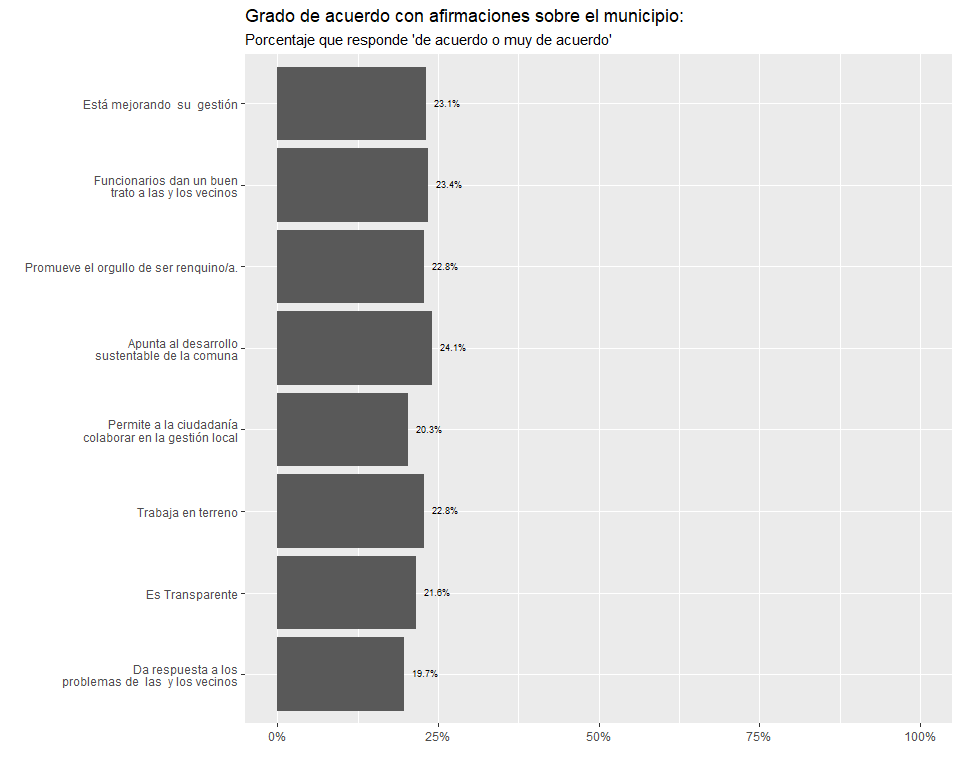
\includegraphics{presentacion-renca_files/figure-latex/eval-gest-1} \end{flushleft}

\hypertarget{b.-evaluaciuxf3n-de-los-servicios-municipales}{%
\subsubsection{b. Evaluación de los servicios
municipales}\label{b.-evaluaciuxf3n-de-los-servicios-municipales}}

\begin{flushleft}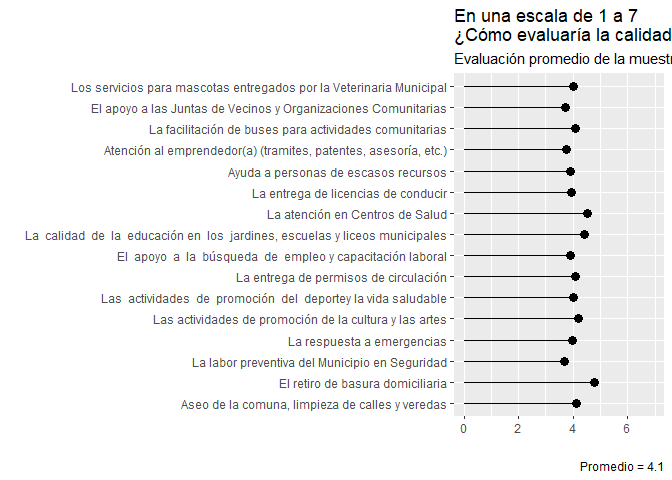
\includegraphics{presentacion-renca_files/figure-latex/eval-serv-1} \end{flushleft}

\hypertarget{c.-evaluaciuxf3n-de-infreaestructura-comunal}{%
\subsubsection{c.~Evaluación de infreaestructura
comunal}\label{c.-evaluaciuxf3n-de-infreaestructura-comunal}}

\begin{flushleft}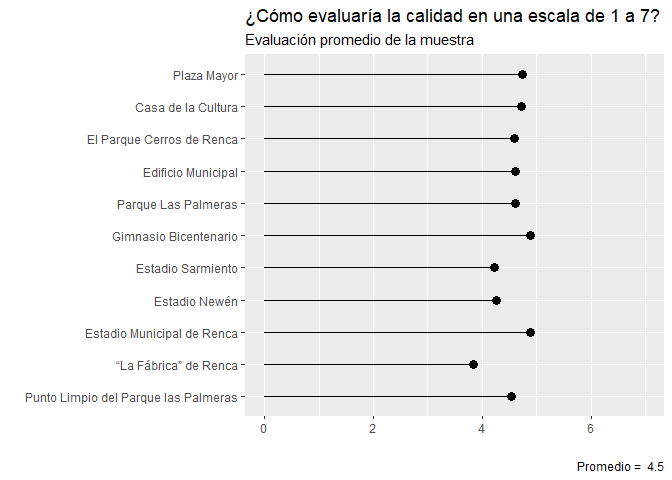
\includegraphics{presentacion-renca_files/figure-latex/eval-infra-1} \end{flushleft}

\hypertarget{d.-evaluaciuxf3n-de-programas-comunales}{%
\subsubsection{d.~Evaluación de programas
comunales}\label{d.-evaluaciuxf3n-de-programas-comunales}}

\begin{flushleft}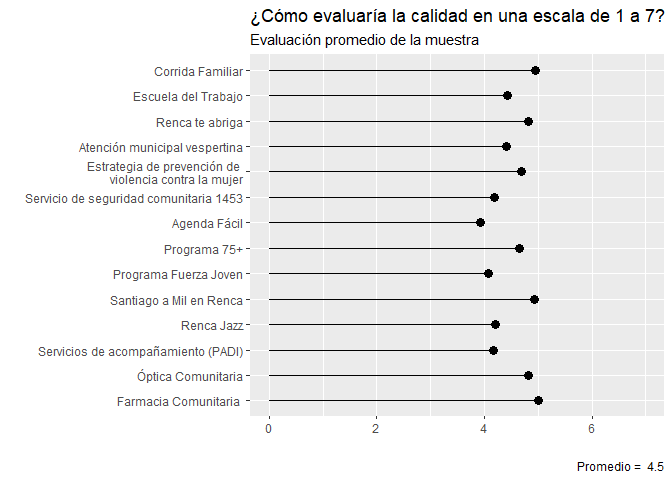
\includegraphics{presentacion-renca_files/figure-latex/eval-progr-1} \end{flushleft}

\hypertarget{evaluaciuxf3n-del-entorno-barrial}{%
\subsection{5.2. Evaluación del entorno
barrial}\label{evaluaciuxf3n-del-entorno-barrial}}

\hypertarget{a.-evaluaciuxf3n-de-los-elementos-del-barrio}{%
\subsubsection{a. Evaluación de los elementos del
barrio}\label{a.-evaluaciuxf3n-de-los-elementos-del-barrio}}

\begin{flushleft}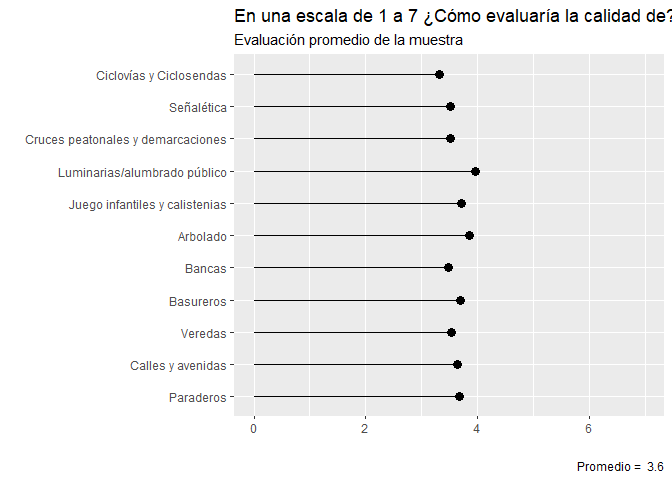
\includegraphics{presentacion-renca_files/figure-latex/eval-barrio-1} \end{flushleft}

\hypertarget{b.-evaluaciuxf3n-de-infraestructura-y-equipamiento-barrial}{%
\subsubsection{b. Evaluación de infraestructura y equipamiento
barrial}\label{b.-evaluaciuxf3n-de-infraestructura-y-equipamiento-barrial}}

\begin{flushleft}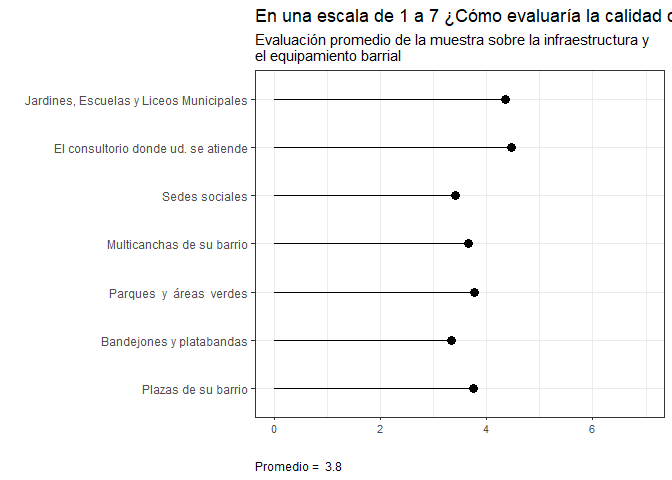
\includegraphics{presentacion-renca_files/figure-latex/nota-barrio-1} \end{flushleft}

\hypertarget{actualidad-y-proyecciuxf3n-comunal}{%
\subsection{5.3 Actualidad y proyección
comunal}\label{actualidad-y-proyecciuxf3n-comunal}}

\hypertarget{a.-fortalezas}{%
\subsubsection{a. Fortalezas}\label{a.-fortalezas}}

\begin{flushleft}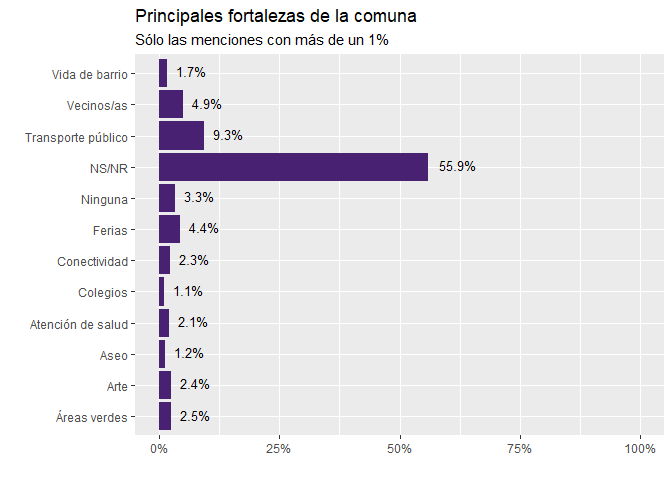
\includegraphics{presentacion-renca_files/figure-latex/fort-renca-1} \end{flushleft}

\hypertarget{b.-problemas}{%
\subsubsection{b. Problemas}\label{b.-problemas}}

\begin{flushleft}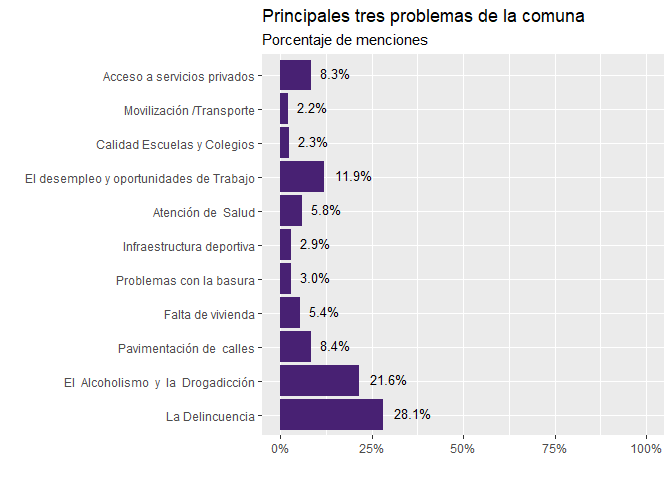
\includegraphics{presentacion-renca_files/figure-latex/prob-renca-1} \end{flushleft}

\hypertarget{c.-proyecciuxf3n-en-tres-auxf1os}{%
\subsubsection{c.~Proyección en tres
años}\label{c.-proyecciuxf3n-en-tres-auxf1os}}

\begin{flushleft}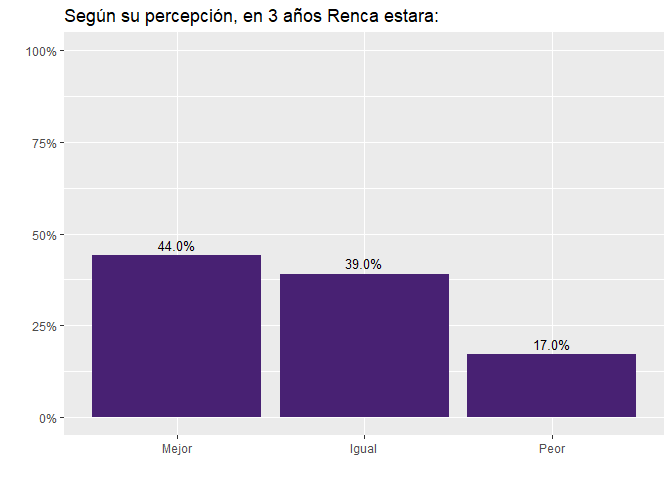
\includegraphics{presentacion-renca_files/figure-latex/proy-renca-1} \end{flushleft}

\end{document}
